%!TEX root = ../Chapter4.tex
\section{Other Saddle-Point Approaches}\label{sec:lgc.sp}

Methods based on approaching the saddle point of the lower bound look promising, one concern about \LG{} (or \LGC{}) could be its computational complexity though. In BAI, the one step complexity of \LG{} is dominated by the computation of the best response for nature, which requires a full matrix inversion. Alternatives that involve rank-1 updates should be considered.

We end this chapter by some more discussions on other possible saddle-point methods.

\subsection{Linear \texorpdfstring{\Track{}}{}}

Although never formally proved, the linear version of \Track seems to be another plausible candidate of being asymptotically optimal provided that a numerical solver for computing the optimal weights exists. Fortunately, the Algorithm~\ref{alg:fw_ab} proposed in Section~\ref{sec:lgc.complexity.complexity} seems to be one. 

\Track remains unchanged in the linear case, since it only cares about tracking the optimal weights. We hereby recall that the \CT rule consists of playing
\[
    \hat\bx \in \argmax_{i\in[K]} \sum_{t=0}^n \omega_i^{\epsilon_t}(\hat\bmu_t)-T_{t,i}\,,
\]
where $\bomega^\epsilon$ is a $L^\infty$ projection of $\bomega^\star$ onto the simplex $\Sigma_K^\epsilon \eqdef \{\bomega\in [\epsilon,1]^K : \sum_{i=1}^K \omega_i = 1\}$. The draw back of \Track is that we need to compute a plug-in estimate of the optimal weights at each stage, which is computationally unfavorable.

\subsection{Saddle-point Frank-Wolfe}
On the other hand, the Frank-Wolfe heuristic in Algorithm~\ref{alg:fw_ab} is an efficient rank-1 solver. It is thus natural to investigate if it can be incorporated into existing algorithms. 

In particular, we can propose two new algorithms by adding the solver on top of \LGapE{} and \LTCC that we call \gls{slgape} and \gls{slt3c} respectively, as shown in Algorithm~\ref{alg:slgape} and Algorithm~\ref{alg:slt3c}. We define a so called \emph{active transductive set} as
\begin{align}\label{def:active_transductive}
    \hat\cY(\bx,\btheta) \eqdef \left\{ \frac{(\bx- \bx')}{\left|(\bx-\bx')\transpose\btheta\right|}: \bx'\in\cX/\big\{\bx\big\}  \right\}\,.
\end{align}

\begin{algorithm}[ht]
\centering
\caption{Algorithm of \SLGapE{}}
\label{alg:slgape}
%\footnotesize
\begin{algorithmic}[1]
    \State {\bfseries Input:} $\delta$
    \State {\bfseries Initialize:} $\mathbf{\tLambda} \leftarrow{} I_d, \mathbf{\Lambda}\leftarrow{} I_d$

   \For{$n \leftarrow 1,2,\cdots$}
        \State $\mathbf{\hat{\bx}}\in\argmax_{\bx\in\cX}  \norm{\bx}_{\mathbf{\Lambda}^{-1} \mathbf{\tLambda} \mathbf{\Lambda}^{-1} }^2$
        \State $\hat{\bx}^{(1)} \leftarrow \argmax_{\bx\in\cX} \bx\transpose\hat\btheta^{\lambda}_n$
        \State $\hat{\bx}^{(2)} \leftarrow \argmax_{\bx\neq\hat{\bx}^{(1)}} (\bx-\hat{\bx}^{(1)})\transpose\hat\btheta^{\lambda}_n + \sqrt{2\beta(n,\delta)}\normm{\hat{\bx}^{(1)}-\bx}_{\bLambda^{-1}}$
        \State $B_n \leftarrow \max_{\bx\neq\hat{\bx}^{(1)}} (\bx-\hat{\bx}^{(1)})\transpose\hat\btheta^{\lambda}_n + \sqrt{2\beta(n,\delta)}\normm{\hat{\bx}^{(1)}-\bx}_{\bLambda^{-1}}$
        \If{$B_n \leq 0$}
            \State \Return $\hat{\bx}^{(1)}$
        \EndIf
        \State $\hat\by \leftarrow{} \dfrac{(\hat{\bx}^{(1)}- \hat{\bx}^{(2)})}{(\hat{\bx}^{(1)}-\hat{\bx}^{(2)})\transpose\btheta}$
        \State $\bLambda\leftarrow{} \mathbf{\Lambda}+ \mathbf{\hat\bx}\mathbf{\hat\bx}\transpose$
		\State $\mathbf{\tLambda} \leftarrow{} \mathbf{\tLambda} + \mathbf{\hat\by}\mathbf{\hat\by}\transpose$
		\State \text{Evaluate arm} $\hat{\bx}$
	    \State \text{Update mean and variance according to \eqref{eq:update_mean} and \eqref{eq:update_variance}}
	    \State $n = n+1$
   \EndFor
\end{algorithmic}
\end{algorithm}

\begin{algorithm}[ht]
\centering
\caption{Sampling rule of \SLTCC{}}
\label{alg:slt3c}
%\footnotesize
\begin{algorithmic}[1]
   \State {\bfseries Initialize:} $\mathbf{\tLambda} \leftarrow{} I_d, \mathbf{\Lambda}\leftarrow{} I_d$

   \For{$n \leftarrow 1,2,\cdots$}
        \State \text{Sample} $\btheta \sim \Pi_n$
        \State $\mathbf{\hat{\bx}}\in\argmax_{\bx\in\cX}  \norm{\bx}_{\mathbf{\Lambda}^{-1} \mathbf{\tLambda} \mathbf{\Lambda}^{-1} }^2$
        \State $\mathbf{\hat{\by}}\in\argmax_{\by\in\hat\cY(\hat\bx,\btheta)}\normm{\by}^2_{\mathbf{\Lambda}^{-1}}$
        \State $\mathbf{\Lambda}\leftarrow{} \mathbf{\Lambda}+ \mathbf{\hat\bx}\mathbf{\hat\bx}\transpose$
		\State $\mathbf{\tLambda} \leftarrow{} \mathbf{\tLambda} + \mathbf{\hat\by}\mathbf{\hat\by}\transpose$
		\State \text{Evaluate arm} $\hat{\bx}$
	    \State \text{Update mean and variance according to \eqref{eq:update_mean} and \eqref{eq:update_variance}}
	    \State $n = n+1$
   \EndFor
\end{algorithmic}
\end{algorithm}

\subsection{Experimental illustrations}

We compare our saddle-point-based algorithms against \LGapE{}. To make a fair comparison, we use always the same exploration rate for all the stopping rules. Indeed the stopping rules are equivalent if they keep the same exploration rate as argued in Appendix~\ref{app:lgc.stopping}. We use the previous hard instance with $c=1$, the results are reported as box plots of average stopping time in Figure~\ref{fig:exp1}.

It seems that they can achieve the same level of empirical performance as \LGapE{}, their theoretical behaviour thus turns out to be an interesting research direction for the future.

\begin{figure}[ht]
    \centering
    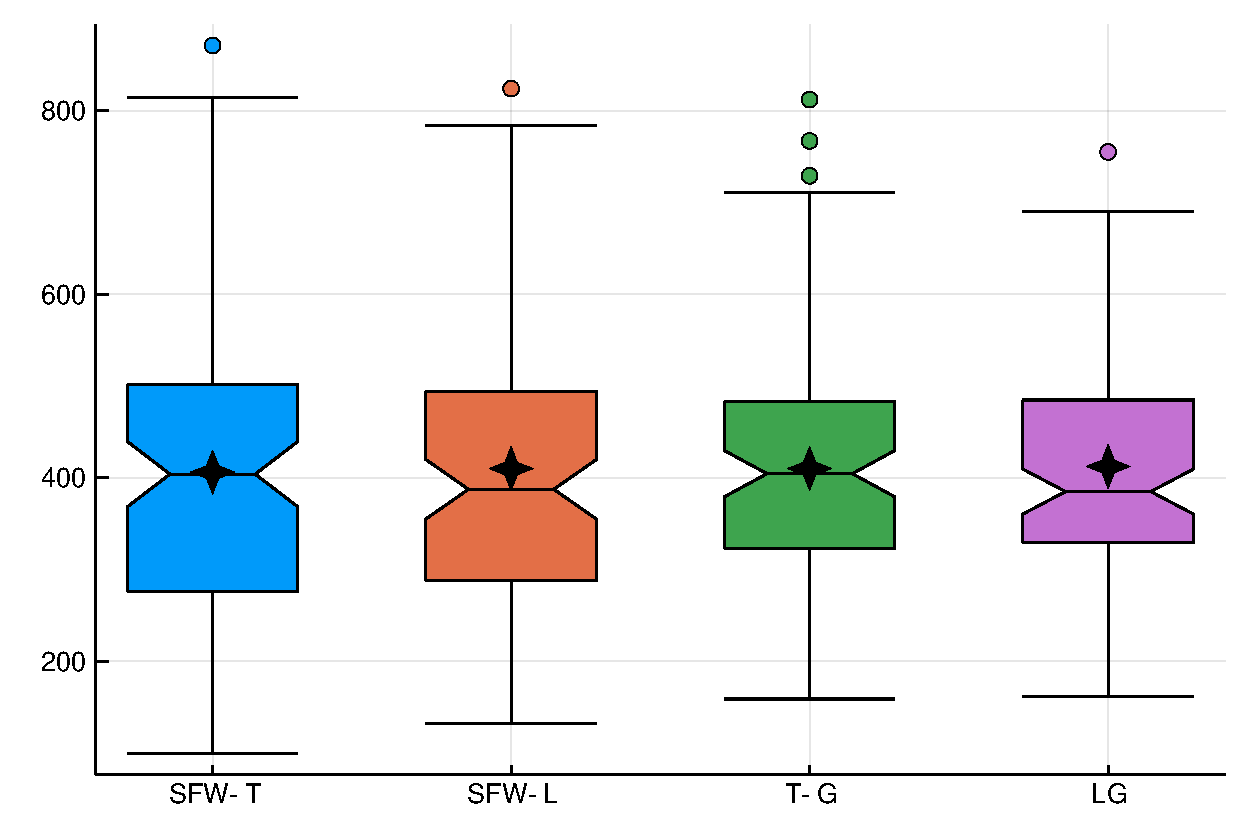
\includegraphics[width=0.33\textwidth]{Chapter4/img/exp_sin_-0000001}
    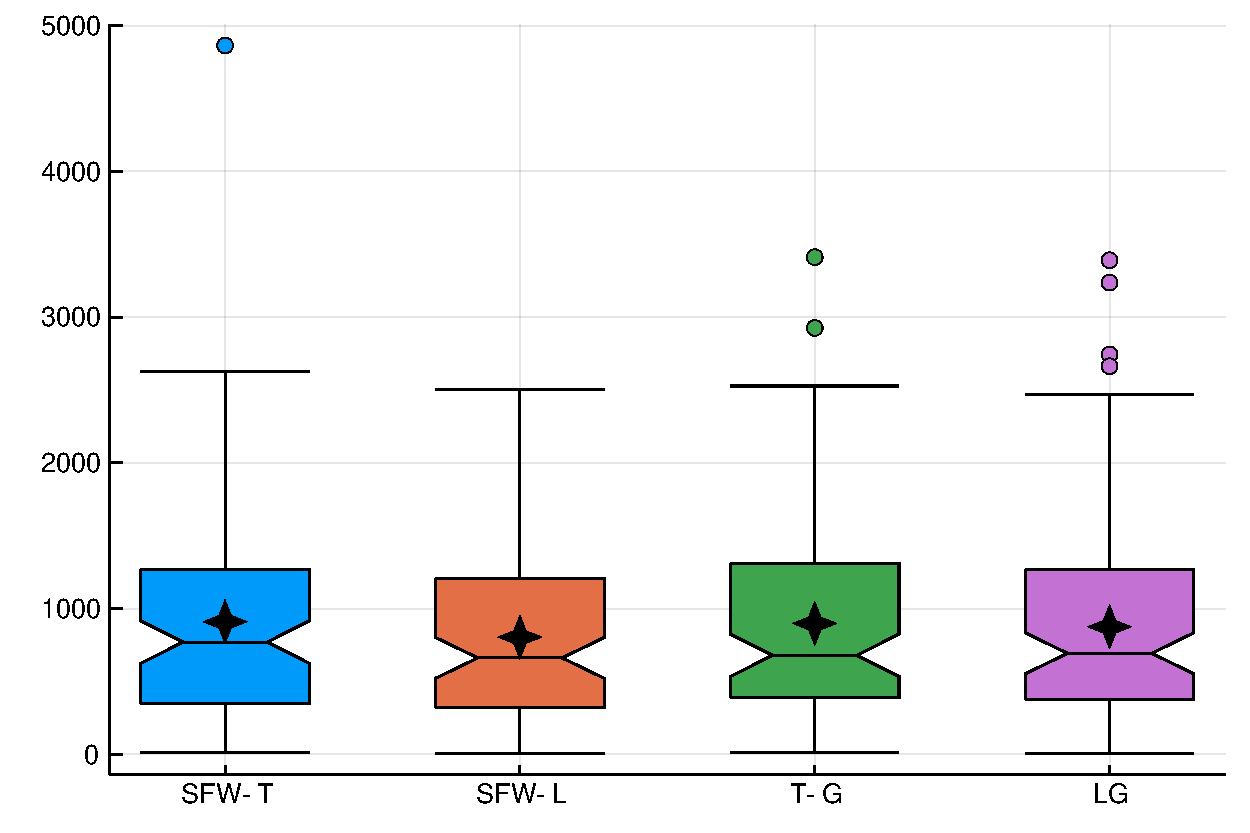
\includegraphics[width=0.33\textwidth]{Chapter4/img/exp_sin_-1}
    \caption{Average stopping time (Left: $d=2,\alpha=\pi/4,\delta=0.0000001$, Right: $d=2,\alpha=0.1,\delta=0.1$), with SFW-T = \SLTCC{}, SFW-L = \SLGapE{}, T-G = \LTCC{}, LG = \LGapE{}.}
    \label{fig:exp1}
\end{figure}
